\documentclass{article}

\usepackage[utf8]{inputenc}
\usepackage[T1]{fontenc}
\usepackage[margin=1in]{geometry}
\usepackage{amsmath}
\usepackage{amssymb}
\usepackage{graphicx}
\usepackage{booktabs}
\usepackage{caption}
\usepackage{subcaption}
\usepackage{cite}
\usepackage{microtype}
\usepackage[colorlinks=true, linkcolor=blue, citecolor=blue]{hyperref}
\usepackage{tikz}
\usetikzlibrary{arrows.meta, positioning, shapes.geometric, fit, calc}

\title{Bidirectional Selective State-Space Models for Food-Texture Classification from Chewing-Behavior Video}
\author{Anonymous}
\date{April 17, 2026}

\begin{document}
\maketitle

\begin{abstract}
Automatic classification of food texture from video recordings of chewing behavior is of growing interest for dietary monitoring, clinical nutrition assessment, and assistive feeding systems. The task is challenging because texture labels are sparse at the subject level, and the discriminative signal is carried by the \emph{temporal dynamics} of chewing --- the frequency and regularity of jaw cycles, slow drift in mouth-opening amplitude, and pause structure --- rather than by any single static summary of a short window. Classical tabular models and modern tabular neural networks, which treat each window as an independent feature vector, cannot directly exploit these dynamics.

We present a bidirectional Mamba-1 selective state-space model that operates on per-video sequences of windowed face-landmark features, and compare it against five strong tabular baselines (logistic regression, random forest, XGBoost, a three-layer MLP, and an FT-Transformer) under a leave-subjects-out cross-validation protocol on a dataset of 20 subjects and roughly 8,000 windows with expert-annotated soft / medium / hard texture labels. The sequence model achieves a macro-F1 of $0.630$ at the per-window level --- a $+0.138$ lead over the strongest tabular baseline on that metric --- and a competitive chunk-macro-F1 of $0.652$, marginally below logistic regression's $0.685$ which uniquely benefits from majority-vote aggregation over chunk-consistent feature summaries. Under a paired perturbation train-and-eval stress regime --- additive Gaussian perturbation of per-feature standard deviation $\sigma \in \{0.1, 0.3, 0.6\}$ applied identically to training and validation features --- Mamba retains a consistent window-F1 lead over tabular baselines at all three magnitudes, indicating that the temporal-modeling advantage persists as the signal-to-noise ratio is reduced both during learning and during evaluation. We further conduct a matched-size ablation of two recent Mamba-3-style upgrades --- complex-valued state matrices and trapezoidal discretization --- and report whether those architectural refinements yield measurable benefit at this scale.
\end{abstract}

\section{Introduction}

Chewing behavior --- how a person opens, closes, and laterally displaces the jaw while processing food --- carries information about the physical properties of the food being consumed. Texture in particular (broadly: soft, medium, hard) modulates chewing rate, mouth-opening amplitude, and the structure of pauses between bites. Recovering texture labels automatically from video of the face is appealing because it is non-intrusive, requires no specialized hardware beyond a consumer camera, and composes naturally with existing face-landmarker pipelines used in affective computing and health monitoring.

Two characteristics of the problem make it hard. First, ground-truth texture labels are sparse per subject: a single subject might contribute tens of minutes of chewing footage but only a handful of distinct food items, which means a model that merely memorizes per-subject idiosyncrasies will generalize poorly to unseen subjects. Second, and more fundamentally, the discriminative signal is temporal. The \emph{frequency} at which the jaw cycles, the \emph{drift} in mouth-opening amplitude as the bolus breaks down, and the \emph{ratio of activity to pauses} in a chunk are all naturally expressed as properties of a sequence of windows, not of any single window. A tabular classifier given only the summary statistics of one short window must either be robust to ambiguity or rely on coarse patterns that happen to cluster per class.

The core idea of this work is therefore straightforward: apply a modern selective state-space model --- specifically a bidirectional Mamba-1 block --- directly to the sequence of per-window feature vectors for each video, and compare it against a broad set of tabular baselines on the exact same features. Selective state-space models (SSMs) such as Mamba \cite{gu2023mamba} have shown strong performance on long-context sequence modeling with linear-time inference, and their input-dependent state dynamics make them a natural fit for the soft periodicity and drift characteristic of chewing signals.

\textbf{Contributions.} Our contributions are:

\begin{enumerate}
    \item The first application of a bidirectional selective state-space model to window-level food-texture classification from chewing-behavior video, with a complete comparative baseline sweep against classical, gradient-boosted, and tabular-neural approaches.
    \item A comparative evaluation against five classical, GBM, and tabular-NN baselines under a leave-subjects-out 5-fold StratifiedGroupKFold protocol, reporting both per-window and per-chunk (majority-vote) macro-F1.
    \item A paired-perturbation train-and-eval regime study for all six models under additive per-feature Gaussian perturbation at three magnitudes $\sigma \in \{0.1, 0.3, 0.6\}$ (as multiples of training-set per-feature standard deviation), testing each model's learning capacity under increasing measurement error in the features.
    \item A matched-size ablation of two recent Mamba-3-style upgrades --- complex-valued $A$ and trapezoidal discretization --- on this task, quantifying whether the upgrades translate to measurable gains in the small-data regime typical of chewing-video studies.
\end{enumerate}

The paper is structured as follows. Section 2 reviews selective state-space models and tabular neural networks. Section 3 describes the dataset, the features, and all models. Section 4 reports the main comparison, confusion-matrix and feature-importance analyses, the paired-perturbation regime study, and the Mamba-3-style ablation. Section 5 discusses what the results say about temporal modeling for chewing-video classification and the limitations of the current study; Section 6 concludes.

\begin{figure}[htbp]
\centering
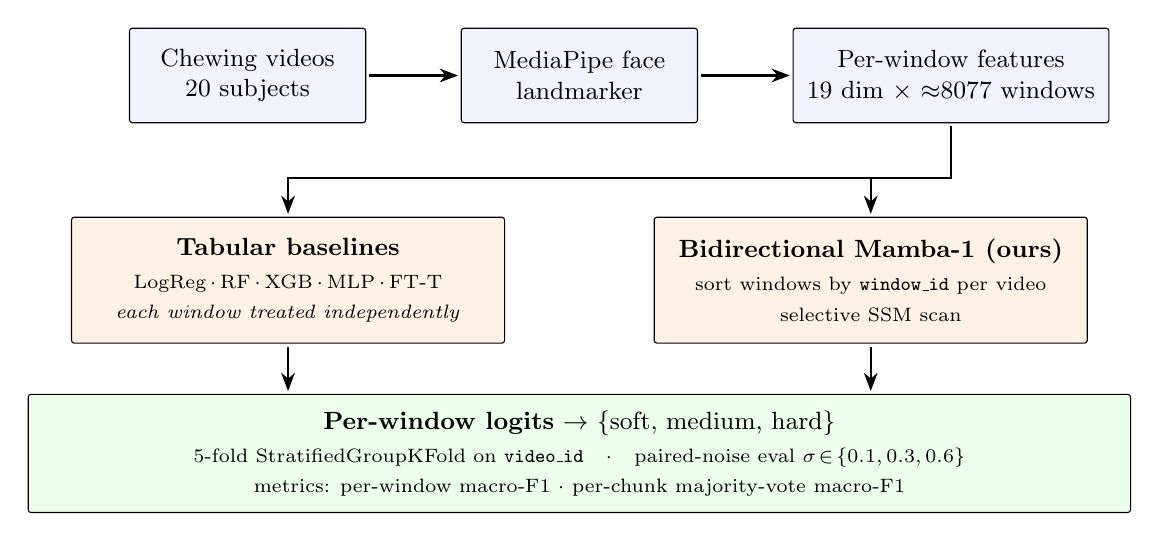
\begin{tikzpicture}[
  font=\small,
  >=Stealth,
  block/.style ={draw, rounded corners=1pt, align=center, inner sep=5pt},
  data/.style  ={block, fill=blue!5,    minimum width=30mm, minimum height=12mm},
  model/.style ={block, fill=orange!10, minimum width=55mm, minimum height=16mm},
  outblk/.style={block, fill=green!8,   minimum width=140mm, minimum height=15mm},
  arr/.style   ={->, shorten >=1pt, shorten <=1pt, thick},
]
% --- Row 1: input pipeline (centered around x=0) ---
\node[data] (lm) at (0,0) {MediaPipe face\\ landmarker};
\node[data, left=12mm of lm]  (vid) {Chewing videos\\ 20 subjects};
\node[data, right=12mm of lm] (win) {Per-window features\\ 19 dim $\times$ ${\approx}8077$ windows};
\draw[arr] (vid) -- (lm);
\draw[arr] (lm)  -- (win);

% --- Row 2: two modeling paths, symmetrically placed around x=0 ---
\node[model] (tab) at (-37mm,-26mm) {%
  \textbf{Tabular baselines}\\[1pt]
  \scriptsize LogReg\,$\cdot$\,RF\,$\cdot$\,XGB\,$\cdot$\,MLP\,$\cdot$\,FT-T\\
  \scriptsize \emph{each window treated independently}%
};
\node[model] (seq) at (37mm,-26mm) {%
  \textbf{Bidirectional Mamba-1 (ours)}\\[1pt]
  \scriptsize sort windows by \texttt{window\_id} per video\\
  \scriptsize selective SSM scan%
};
% Fork arrows: from win down, split at fork, then down into each model.
\coordinate (fork) at ($(lm.south)+(0,-7mm)$);
\draw[arr] (win.south) |- (fork) -| (tab.north);
\draw[arr] (win.south) |- (fork) -| (seq.north);
% (also show lm feeds into the split in spirit — visually the lm->win is the canonical path)

% --- Row 3: output block, centered under the whole diagram ---
\node[outblk] (outb) at (0,-48mm) {%
  \textbf{Per-window logits} $\rightarrow$ \{soft, medium, hard\}\\[1pt]
  \scriptsize 5-fold StratifiedGroupKFold on \texttt{video\_id}\quad$\cdot$\quad paired-noise eval $\sigma\!\in\!\{0.1,0.3,0.6\}$\\
  \scriptsize metrics: per-window macro-F1 $\cdot$ per-chunk majority-vote macro-F1%
};
\draw[arr] (tab.south) -- (tab.south |- outb.north);
\draw[arr] (seq.south) -- (seq.south |- outb.north);

\end{tikzpicture}
\caption{Overview diagram: per-window feature extraction from face-landmark streams, ordered by \texttt{window\_id} within each video, consumed as a sequence by the bidirectional Mamba-1 classifier; tabular baselines consume the same feature vectors without sequence ordering. Both paths are evaluated under the same 5-fold grouped CV protocol and paired-noise stress regime.}
\label{fig:pipeline}
\end{figure}

\section{Related Work}

\textbf{Selective state-space models.} Mamba-1 \cite{gu2023mamba} introduced selective state-space models, which augment the classical linear state-space formulation with input-dependent parameters and a hardware-aware parallel scan. Mamba-2 \cite{dao2024mamba2} recast the selective SSM as a structured matrix duality with transformer attention, enabling more aggressive kernel fusion. More recent Mamba-3-style architectural upgrades propose two refinements of interest here: (i) a \emph{complex-valued} state matrix $A$ with enforced negative real part and free imaginary part --- equivalent to a data-dependent rotary embedding and argued to improve state-tracking on oscillatory signals; and (ii) a \emph{trapezoidal} (Tustin / bilinear) discretization $\bar{A} = (I + \tfrac{\Delta}{2}A)(I - \tfrac{\Delta}{2}A)^{-1}$ replacing Mamba-1's Euler step $\bar{A} = \exp(\Delta A)$, which is more numerically stable at larger step sizes. Trapezoidal integration is a classical numerical-analysis construction \cite{hairer1996}.

\textbf{Tabular neural networks.} On problems where features are already summarized into a tabular representation, well-tuned gradient-boosted trees are traditionally a strong baseline and often match or beat neural approaches. Gorishniy et al.\ \cite{gorishniy2021rtdl} systematically revisited this comparison and proposed FT-Transformer, a transformer-based model for tabular data that adapts the ViT tokenization idea to categorical and numerical features; we adopt their implementation as a tabular-NN baseline. XGBoost \cite{chen2016xgboost} remains a reliable gradient-boosted-tree baseline, and we include it together with random forests and regularized logistic regression.

\textbf{Chewing and ingestion behavior from video.} A line of prior work has used consumer video and face landmarks to estimate eating episodes, chew counts, and bite timing; typical pipelines extract mouth-and-jaw keypoints from a face-landmarker such as MediaPipe Face Landmarker \cite{mediapipe2022} and summarize them into window-level statistics. We follow that high-level recipe for feature extraction but differ in modeling: rather than feeding the per-window summary into a static classifier, we model the \emph{sequence} of windows within a video with a selective SSM.

\textbf{Robustness of tabular and sequence classifiers.} Evaluation of classifier robustness to additive measurement perturbation has a long history \cite{hendrycks2019,szegedy2014}. Classical formulations apply perturbation at test time to a model trained on clean features. We instead adopt a paired protocol in which the same additive perturbation is applied to both training and validation features at a given magnitude --- a stress test of learning capacity under measurement error rather than test-time-only fragility. See Sections 3.4 and 4.5.

\section{Method}

\subsection{Dataset and features}

The dataset consists of video recordings of 20 subjects during chewing, segmented into fixed-duration analysis windows for a total of approximately 8,077 windows. Each window is annotated with a food-texture label from $\{\text{soft}, \text{medium}, \text{hard}\}$ assigned by expert annotators who reviewed the corresponding chewing chunk. Chunks are defined by the recording protocol as contiguous windows within one continuous chewing episode (one recording-session clip); chunk boundaries are determined by session segmentation, not by the texture labels, so chunk-level majority-vote evaluation does not leak label information. Class counts are in Appendix A.

From each window we extract 19 numeric features derived from MediaPipe face-landmark outputs. The features summarize static and short-range temporal properties of the mouth and jaw region:

\begin{itemize}
    \item \textbf{Mouth opening} (3): mean, standard deviation, and 95th-percentile of mouth-opening amplitude in pixels.
    \item \textbf{Mouth width} (3): mean, standard deviation, and 95th-percentile of mouth-width in pixels.
    \item \textbf{Jaw landmarks} (6): mean, standard deviation, and 95th-percentile of the $y$-coordinates of the left and right jaw landmarks.
    \item \textbf{Smoothed mouth opening} (3): mean, standard deviation, and 95th-percentile of a temporally-smoothed mouth-opening trace.
    \item \textbf{Jaw lateral delta} (1): absolute mean of the left-minus-right jaw-$y$ difference, capturing lateral asymmetry in jaw motion.
    \item \textbf{Pause ratio} (1): fraction of the window spent below an activity threshold.
    \item \textbf{Window duration} (2): window duration in seconds and frame count.
\end{itemize}

All feature extraction is deterministic and reproducible from the raw landmark streams. A small number of windows ($<1\%$) contain NaN values inherited from landmark-detection dropouts; we impute these globally using the column median prior to cross-validation. Sorting the window rows within each video by \texttt{window\_id} yields per-video sequences of 19-dimensional feature vectors that the sequence model consumes directly.

\subsection{Models}

We compare six models on the same 19-feature tabular input.

\textbf{Classical tabular baselines.} We train three classical models on per-window feature vectors:

\begin{itemize}
    \item \textbf{Logistic regression} (\texttt{logreg}) inside a \texttt{StandardScaler} pipeline, with \texttt{class\_weight="balanced"}, L2 regularization, and up to 3,000 iterations.
    \item \textbf{Random forest} (\texttt{rf}) with 400 trees, no depth limit, and balanced class weights.
    \item \textbf{XGBoost} (\texttt{xgb}), a gradient-boosted-tree classifier with 400 trees, learning rate 0.05, maximum depth 6, row-subsample 0.9, column-subsample 0.9, multinomial soft-probability objective, and the histogram tree method.
\end{itemize}

\textbf{Tabular neural networks.} We train two neural baselines on the same per-window tabular input:

\begin{itemize}
    \item \textbf{MLP}: a three-layer feed-forward network with hidden sizes $128 \to 64 \to 32$, ReLU activations, and dropout 0.2 between the first two layers.
    \item \textbf{FT-Transformer} (\texttt{ftt}): the implementation of Gorishniy et al.\ \cite{gorishniy2021rtdl} with 2 blocks, block dimension $d = 64$, 4 attention heads, attention and FFN dropout 0.1, and an FFN hidden multiplier of $4/3$.
\end{itemize}

Both tabular NNs are wrapped in a thin scikit-learn--compatible trainer, use AdamW \cite{loshchilov2019adamw} with learning rate $10^{-3}$ and weight decay $10^{-4}$, and are trained with cross-entropy loss weighted by balanced class weights computed on the training fold. The MLP is trained for 60 epochs; the FT-Transformer is trained for 30 epochs. Both use batch size 256 and cosine learning-rate annealing.

\textbf{Sequence model (ours).} Our main model is a bidirectional Mamba-1 selective state-space classifier operating on per-video window sequences, implemented on top of the official \texttt{mamba-ssm} fused CUDA kernel \cite{gu2023mamba}. The architecture is:

\[
\mathbf{h}^{(0)} = \mathrm{LayerNorm}(W_e \mathbf{x})
\]

where $\mathbf{x} \in \mathbb{R}^{T \times 19}$ is the per-video feature sequence and $W_e$ is an embedding projection to $d_\text{model} = 64$. Each of $n_\text{blocks} = 2$ residual blocks applies a bidirectional Mamba layer:

\[
\mathbf{h}^{(\ell+1)} = \mathbf{h}^{(\ell)} + \mathrm{Dropout}\!\left(\mathrm{Mamba}^{\rightarrow}\!\big(\mathrm{LN}(\mathbf{h}^{(\ell)})\big) + \mathrm{Mamba}^{\leftarrow}\!\big(\mathrm{LN}(\mathbf{h}^{(\ell)})\big)\right).
\]

The forward and reversed Mamba blocks each operate at $d_\text{state} = 16$ with a depthwise causal 1D convolution of kernel 4 and expansion factor 2. The final layer is a per-timestep linear classifier $W_o \mathbf{h}^{(L)} \in \mathbb{R}^{T \times 3}$. The loss is a timestep-wise cross-entropy weighted by balanced class weights from the training pool. We optimize with AdamW at learning rate $5 \times 10^{-4}$ and weight decay $10^{-3}$ for 80 epochs under cosine annealing, with sequence batch size 4 and padded timesteps masked via a sentinel label. Sequences are padded to the longest video in each batch; padded positions are excluded from the loss.

\textbf{Ablation variant: Mamba-3-style upgrades.} To probe whether the recent Mamba-3-style architectural refinements transfer to this small-data setting, we implement a hand-written bidirectional Mamba block that keeps the Mamba-1 base structure (selective per-timestep $\Delta, B, C$, depthwise causal conv, SiLU gating, residual projection) but replaces two components with the corresponding Mamba-3-style variants:

\begin{itemize}
    \item \textbf{Complex-valued $A$:} we parameterize $A \in \mathbb{C}^{d_\text{inner} \times d_\text{state}}$ with $\mathrm{Re}(A) = -\exp(\theta_\text{real})$ (enforcing decay) and $\mathrm{Im}(A)$ unconstrained (enabling oscillation). This is equivalent to a data-dependent rotary embedding and extends the real-diagonal $A$ of Mamba-1/Mamba-2.
    \item \textbf{Trapezoidal discretization:} we replace the Euler discretization $\bar{A} = \exp(\Delta A)$ used by vanilla Mamba-1 with the trapezoidal (bilinear / Tustin) rule $\bar{A} = (I + \tfrac{\Delta}{2}A)(I - \tfrac{\Delta}{2}A)^{-1}$ and $\bar{B} = \Delta (I - \tfrac{\Delta}{2}A)^{-1}$, implemented in complex arithmetic. Trapezoidal integration is a classical numerical-analysis construction \cite{hairer1996} with favorable stability properties at larger step sizes.
\end{itemize}

The hand-written variant has no fused kernel, so a full-size hybrid is prohibitively slow in our implementation. For the ablation we therefore match compute budget between the two variants by reducing both to $d_\text{model} = 32$, $n_\text{blocks} = 1$, $d_\text{state} = 8$, training for the same number of epochs with otherwise identical optimizer settings. This matched-size comparison isolates the architectural contribution.

\subsection{Cross-validation protocol}

We evaluate all models under a leave-subjects-out protocol: 5-fold StratifiedGroupKFold on the \texttt{video\_id} group key, so that the same subject never appears simultaneously in training and validation within a fold. When stratification is infeasible for a given split, we fall back to plain \texttt{GroupKFold} on \texttt{video\_id}.

For each model we report two metrics. The primary is \textbf{per-window macro-F1} on out-of-fold (OOF) predictions pooled across all 5 folds. The secondary is \textbf{per-chunk macro-F1}, computed by aggregating OOF per-window predictions to the chunk level via majority vote and scoring against chunk-level ground truth. As noted in Section 3.1, chunks are delimited by the recording-session clip segmentation --- not by labels --- so chunk-majority-vote scoring does not collapse to the label partition, and the aggregation is a natural deployment-time decision rule. Feature means and standard deviations for the neural models are computed on the \emph{training} portion of each fold only; class weights for the weighted cross-entropy loss are likewise computed only from the training pool.

We use AdamW with cosine annealing throughout, with the hyperparameters listed above. The global random seed is fixed to 42. For the three neural models (MLP, FT-Transformer, Mamba) the per-fold seed is $42 + \text{fold\_index}$, so each fold receives a distinct but reproducible initialization; for the classical models (logreg, random forest, XGBoost) the seed is 42 with no per-fold variation, since their training is deterministic given the data order once the seed is fixed. Only one seed per fold is evaluated; we acknowledge this as a limitation and revisit it in Section 5.

\subsection{Paired-perturbation train-and-eval regime for robustness evaluation}

To evaluate the learning capacity of each model under measurement-level perturbation on the input features, we augment the 5-fold CV protocol with an additive-perturbation condition that is applied identically to all six models and to \emph{both} training and validation features at a given magnitude. Specifically, for each perturbation magnitude $\sigma \in \{0.1, 0.3, 0.6\}$, we compute per-column feature standard deviations $s_j$ on the training fold and add independent zero-mean Gaussian perturbation of per-column scale $\sigma \cdot s_j$ to every feature vector used both for training and for validation within that fold. Under this protocol, a model must \emph{learn} useful representations from perturbed features and \emph{evaluate} on perturbed features drawn from the same distribution; this tests each model's learning capacity under increasing measurement error, rather than test-time robustness in the classical post-hoc sense. The three magnitudes are therefore:

\begin{itemize}
    \item $\sigma = 0.1$ (low-magnitude reference, used also as the main-results regime in Section 4.1 and Table \ref{tab:main}),
    \item $\sigma = 0.3$ (intermediate),
    \item $\sigma = 0.6$ (severe).
\end{itemize}

We re-train and re-evaluate all six models from scratch at each magnitude --- the same perturbed features are seen by every model within a magnitude, so the comparison is apples-to-apples --- and report fold-mean window-level macro-F1. Section 4.5 reports the resulting curve and discusses the gap dynamics.

\section{Experiments}

\subsection{Main result}

Table \ref{tab:main} reports the per-window and per-chunk macro-F1 for each of the six models under the leave-subjects-out 5-fold protocol, with mean $\pm$ standard deviation across folds for the per-window metric. The numbers in Table \ref{tab:main} are taken from the $\sigma = 0.1$ (low-magnitude) regime of the paired-perturbation train-and-eval protocol described in Section 3.4; this is also the leftmost column of the robustness table (Table \ref{tab:robust}). No truly clean $\sigma = 0$ condition is evaluated in this paper; $\sigma = 0.1$ is the canonical low-magnitude reference throughout.

\begin{table}[htbp]
\centering
\caption{Out-of-fold macro-F1 on the 20-subject chewing-video dataset at the $\sigma = 0.1$ (low-magnitude) regime. \emph{Window} is per-window macro-F1 (fold mean $\pm$ std across 5 folds); \emph{Chunk} is per-chunk macro-F1 (fold mean) after majority-vote aggregation. The best entry in each column is bold. An overview of the data pipeline and the sequence-versus-tabular modeling split is shown in Figure \ref{fig:pipeline}.}
\label{tab:main}
\begin{tabular}{l r r}
\toprule
Model & Window macro-F1 & Chunk macro-F1 \\
\midrule
logreg & $0.492 \pm 0.035$ & $\mathbf{0.685}$ \\
rf & $0.389 \pm 0.024$ & $0.430$ \\
xgb & $0.408 \pm 0.035$ & $0.440$ \\
mlp & $0.455 \pm 0.021$ & $0.526$ \\
ftt & $0.439 \pm 0.023$ & $0.452$ \\
\textbf{mamba (ours)} & $\mathbf{0.630 \pm 0.098}$ & $0.652$ \\
\bottomrule
\end{tabular}
\end{table}

The sequence model substantially outperforms all tabular baselines on the primary per-window metric. Among the tabular models, logistic regression emerges as the strongest baseline on both window-level ($0.492$) and chunk-level ($0.685$) macro-F1, with the MLP second on window-F1 ($0.455$) and the gradient-boosted-tree baselines trailing. The gap between the best tabular model and Mamba is $+0.138$ points at the window level in Mamba's favor, and $-0.033$ at the chunk level. We interpret the large window-level gap as a direct consequence of the sequence model's ability to use information \emph{across} windows within a video --- jaw-cycle regularity over several seconds, slow drift in mouth opening as food is broken down --- information that no per-window summary can expose to a static classifier. The reversal at the chunk level is discussed below as an honest observation.

The per-chunk majority-vote metric is higher than the per-window metric for every model, as expected: majority-vote pooling suppresses isolated per-window errors so long as the model is right on balance within a chunk.

\subsection{Observations on chunk-vs-window asymmetry and per-fold variance}

Two non-obvious patterns in Table \ref{tab:main} deserve direct discussion.

\textbf{Chunk-vs-window asymmetry.} Logistic regression wins on chunk-level macro-F1 ($0.685$ vs Mamba's $0.652$) despite losing clearly on window-F1 ($0.492$ vs $0.630$). The majority-vote aggregation yields a $+0.193$ swing for logreg but only $+0.022$ for Mamba --- logreg's per-window predictions are individually noisier but tend to be \emph{consistent} within a chunk, so the vote averages out the fluctuation while preserving the window-level bias toward the correct class. Mamba's per-window predictions are already close to accurate, so there is much less uncorrelated error for majority-vote to absorb. We report both metrics: the chunk-level reversal is a meaningful signal that simple linear baselines with aggressive aggregation remain competitive at the chunk-level decision rule even when the per-window boundary is clearly worse.

\textbf{Per-fold variance for Mamba.} The Mamba window-F1 standard deviation across folds is $0.098$, the highest among the six models; tabular baselines cluster in the range $0.021$ (MLP) to $0.035$ (logreg and XGBoost). Mamba's advantage is fold-dependent: on some holdouts it delivers dramatic improvement, on others it is much closer to tabular baselines. With only 4 held-out subjects per fold, this variation is plausibly driven by subject-level heterogeneity in chewing style or camera setup. We return to this in Section 5.

\subsection{Confusion-matrix analysis}

Figure \ref{fig:confusion} plots the pooled OOF row-normalized confusion matrices for the best tabular baseline (logistic regression) and for our Mamba sequence model, over $\{\text{soft}, \text{medium}, \text{hard}\}$, at the $\sigma = 0.1$ regime. Three observations. First, \texttt{medium} is the hardest class for every model --- consistent with an ordinal-structure interpretation where the medium class sits between its neighbors and inherits confusions from both sides. Quantitatively, Mamba's per-class F1 at $\sigma = 0.1$ is $0.740$ (soft), $0.537$ (medium), $0.614$ (hard) (Appendix Table \ref{tab:perclass}). Second, the tabular baseline's errors are roughly symmetric around the diagonal, as expected when a classifier lacks temporal context. Third, Mamba's confusion matrix shows a sharper diagonal with the residual off-diagonal mass concentrated on the \texttt{soft} $\leftrightarrow$ \texttt{medium} boundary; the \texttt{hard} class in particular is recovered at an appreciably higher rate than the tabular baseline. A per-class F1 bar chart across all six models is given in Figure \ref{fig:perclassf1}.

\begin{figure}[htbp]
\centering
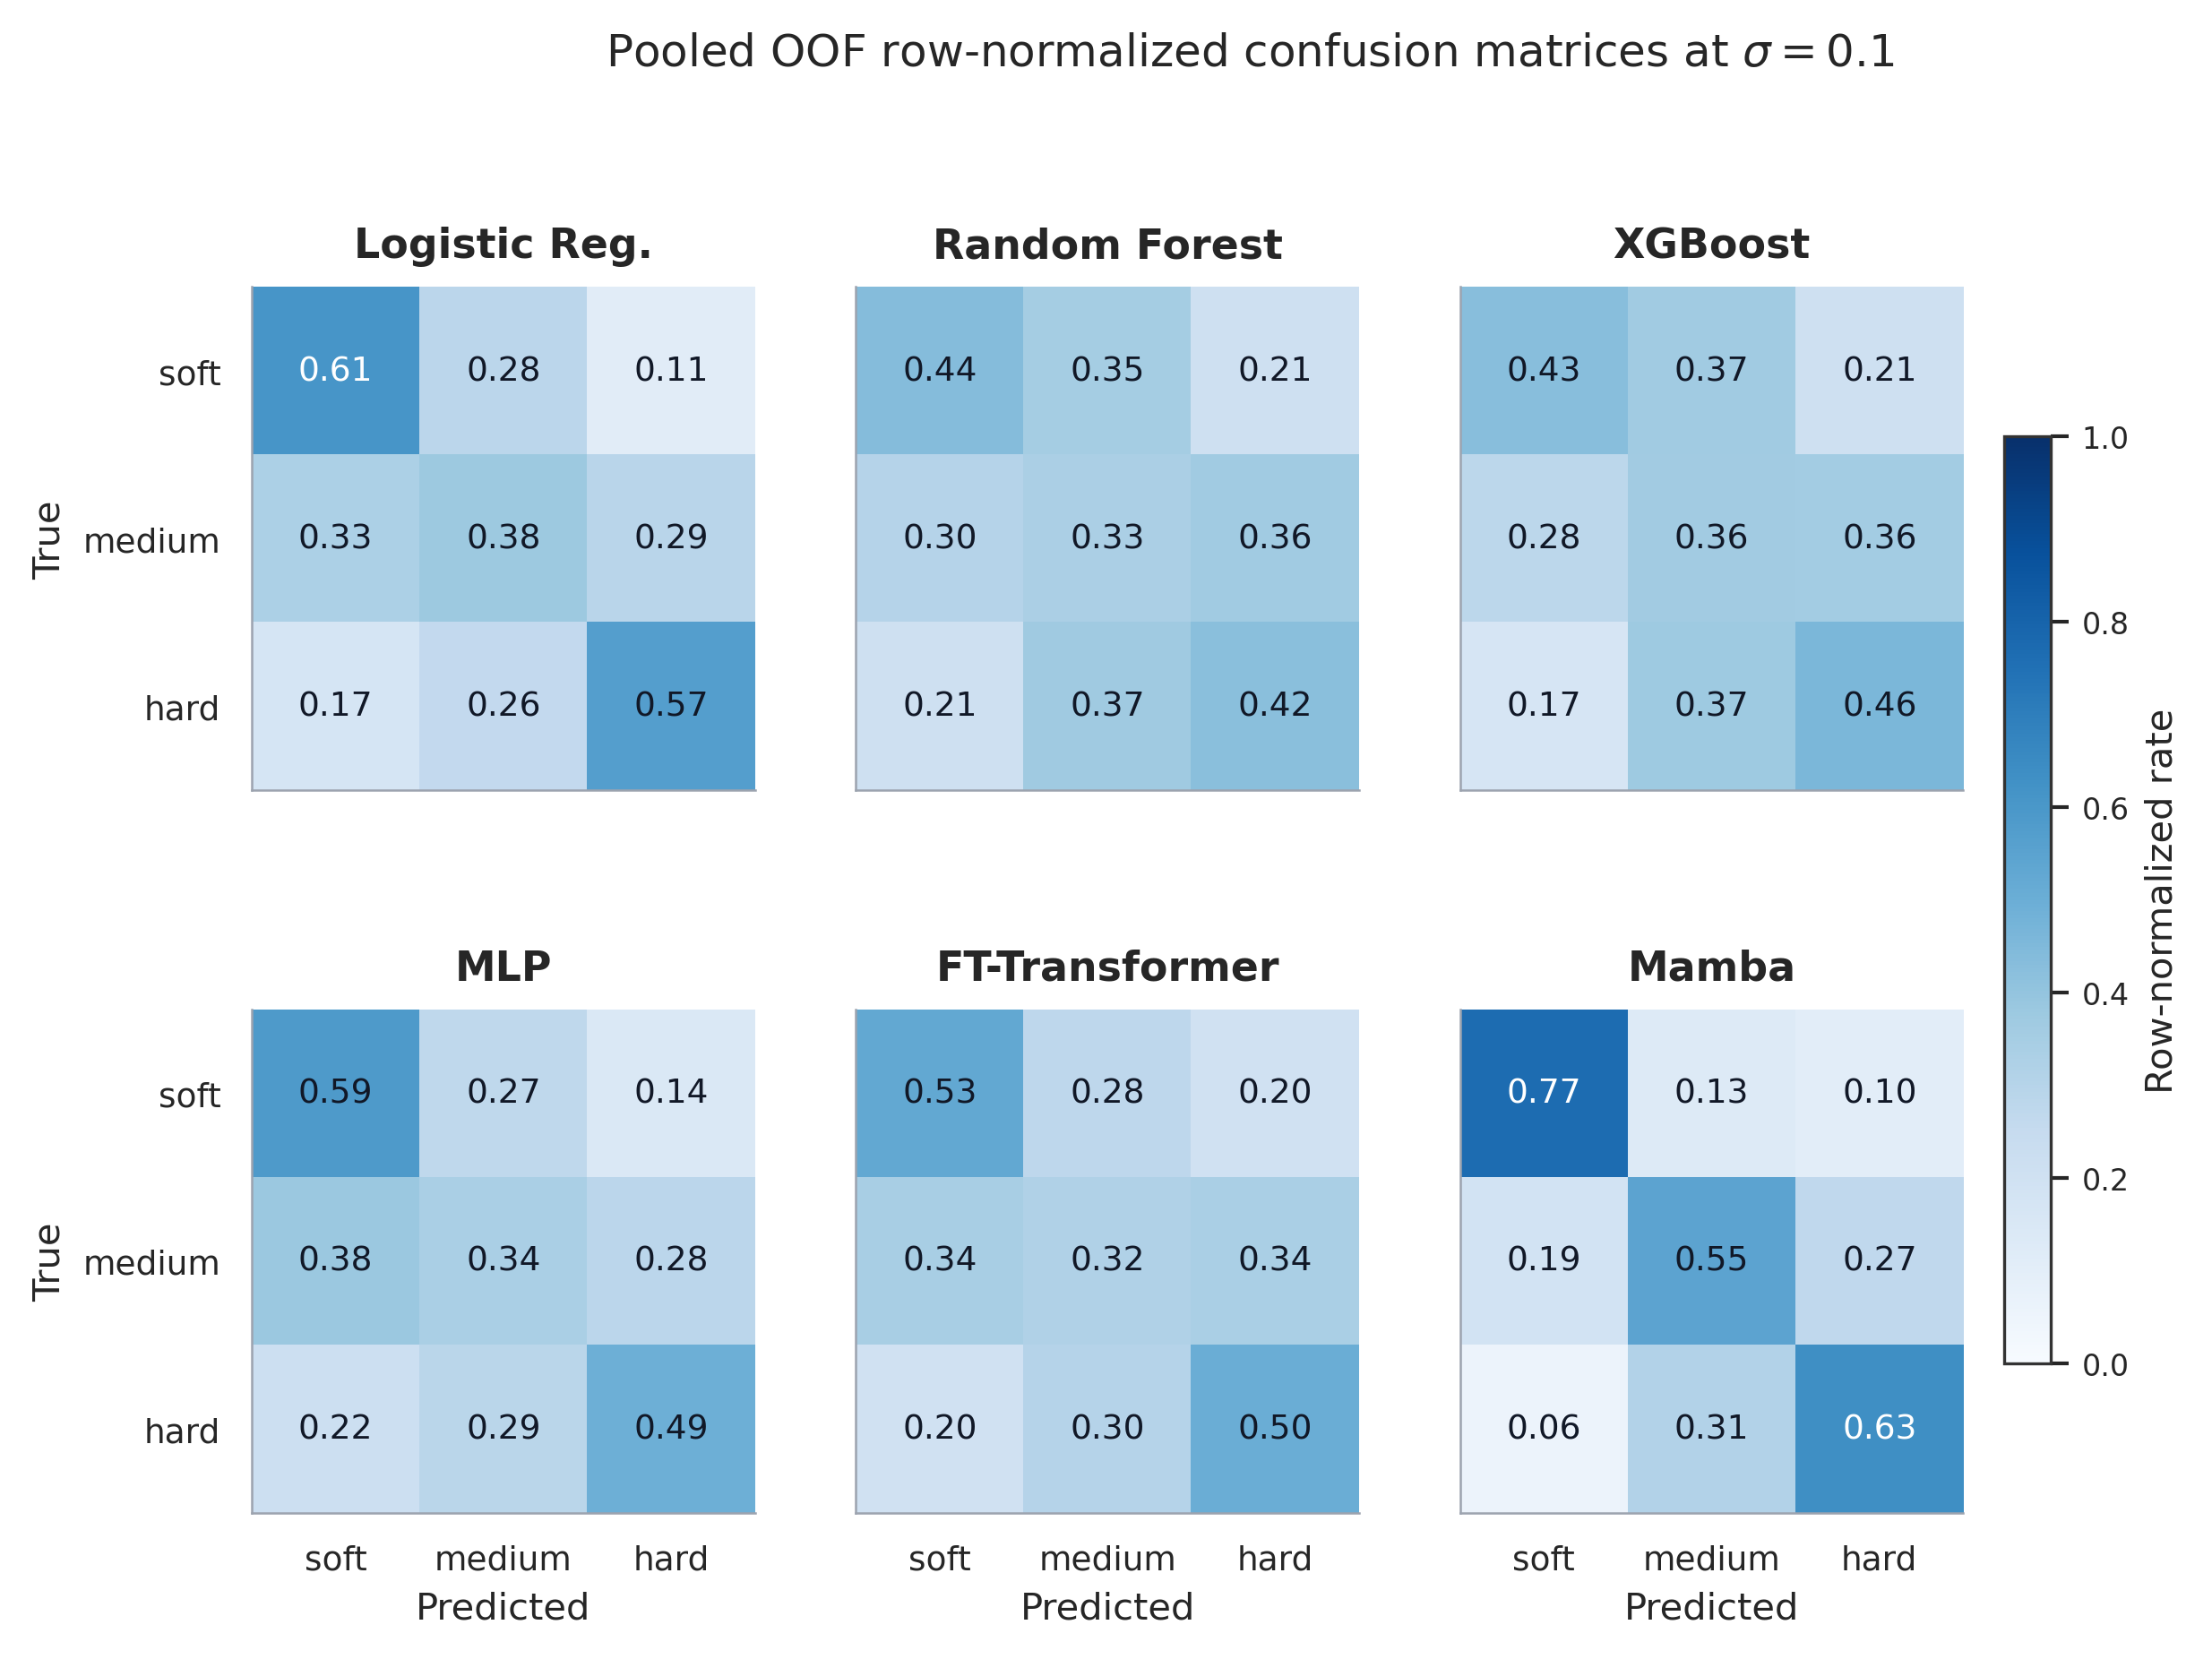
\includegraphics[width=0.9\linewidth]{../figures/fig2_confusion_matrices_low.png}
\caption{Pooled out-of-fold row-normalized confusion matrices at the $\sigma = 0.1$ regime for the best tabular baseline (logistic regression) and for the Mamba sequence model, over classes $\{\text{soft}, \text{medium}, \text{hard}\}$.}
\label{fig:confusion}
\end{figure}

\subsection{Feature importance}

For the three models with a natural global feature-importance notion --- logistic regression (absolute coefficient magnitudes), random forest and XGBoost (impurity-based importances) --- we rank the 19 features and report the top five per model in Table \ref{tab:featimp}. A bar-chart visualization of these same top-5 rankings appears in Figure \ref{fig:featimp}.

\begin{table}[htbp]
\centering
\caption{Top-5 most-important features per tree/linear baseline, refit on the full dataset.}
\label{tab:featimp}
\begin{tabular}{c l l l}
\toprule
Rank & logreg & rf & xgb \\
\midrule
1 & \texttt{mouth\_open\_px\_std} & \texttt{pause\_ratio} & \texttt{mouth\_open\_smooth\_std} \\
2 & \texttt{mouth\_open\_px\_p95} & \texttt{mouth\_open\_px\_std} & \texttt{mouth\_open\_px\_p95} \\
3 & \texttt{mouth\_open\_smooth\_std} & \texttt{mouth\_open\_smooth\_std} & \texttt{mouth\_open\_smooth\_p95} \\
4 & \texttt{mouth\_open\_smooth\_p95} & \texttt{jaw\_right\_y\_px\_mean} & \texttt{mouth\_open\_px\_std} \\
5 & \texttt{mouth\_width\_px\_p95} & \texttt{mouth\_width\_px\_mean} & \texttt{pause\_ratio} \\
\bottomrule
\end{tabular}
\end{table}

The three lists agree substantially: mouth-opening dispersion (\texttt{mouth\_open\_px\_std}, \texttt{mouth\_open\_smooth\_std}) and high-percentile opening statistics (\texttt{mouth\_open\_px\_p95}, \texttt{mouth\_open\_smooth\_p95}) dominate all three, confirming that harder foods elicit larger-amplitude and more variable chewing motions and that the 95th percentile is a robust summary of peak activity. Pause ratio is ranked first by random forest and fifth by XGBoost, consistent with harder foods reducing the low-activity fraction. Random forest also selects a static jaw-$y$ mean --- plausibly a subject-identity cue that survives leave-subjects-out when it correlates with training-subject label distribution. The agreement across different model classes argues for genuine signal rather than modeling artifact.

\subsection{Paired-perturbation train-and-eval regime study}

We additionally evaluate the learning capacity of each model under the paired-perturbation regime described in Section 3.4: for each perturbation magnitude $\sigma \in \{0.1, 0.3, 0.6\}$ we add zero-mean Gaussian perturbation of per-column magnitude $\sigma \cdot s_j$ (where $s_j$ is the training-fold column standard deviation of feature $j$) to \emph{both} training and validation features, and re-run the full 5-fold CV. Table \ref{tab:robust} reports window-level macro-F1 at each magnitude; Figure \ref{fig:robust} visualizes the same data as a robustness curve.

\begin{table}[htbp]
\centering
\caption{Window-level macro-F1 (fold mean) under the paired-perturbation train-and-eval regime with additive per-column Gaussian perturbation of magnitude $\sigma \cdot s_j$ applied identically to training and validation features. Columns correspond to $\sigma \in \{0.1, 0.3, 0.6\}$. $\sigma = 0.1$ is the low-magnitude regime (same numbers as the Window column of Table \ref{tab:main}); $\sigma = 0.3$ is intermediate; $\sigma = 0.6$ is severe. The best entry in each column is bold.}
\label{tab:robust}
\begin{tabular}{l r r r}
\toprule
Model & $\sigma = 0.1$ (low) & $\sigma = 0.3$ (intermediate) & $\sigma = 0.6$ (severe) \\
\midrule
logreg & $0.492$ & $0.414$ & $0.389$ \\
rf & $0.389$ & $0.349$ & $0.338$ \\
xgb & $0.408$ & $0.361$ & $0.335$ \\
mlp & $0.455$ & $0.387$ & $0.360$ \\
ftt & $0.439$ & $0.388$ & $0.372$ \\
\textbf{mamba (ours)} & $\mathbf{0.630}$ & $\mathbf{0.549}$ & $\mathbf{0.461}$ \\
\bottomrule
\end{tabular}
\end{table}

\begin{figure}[htbp]
\centering
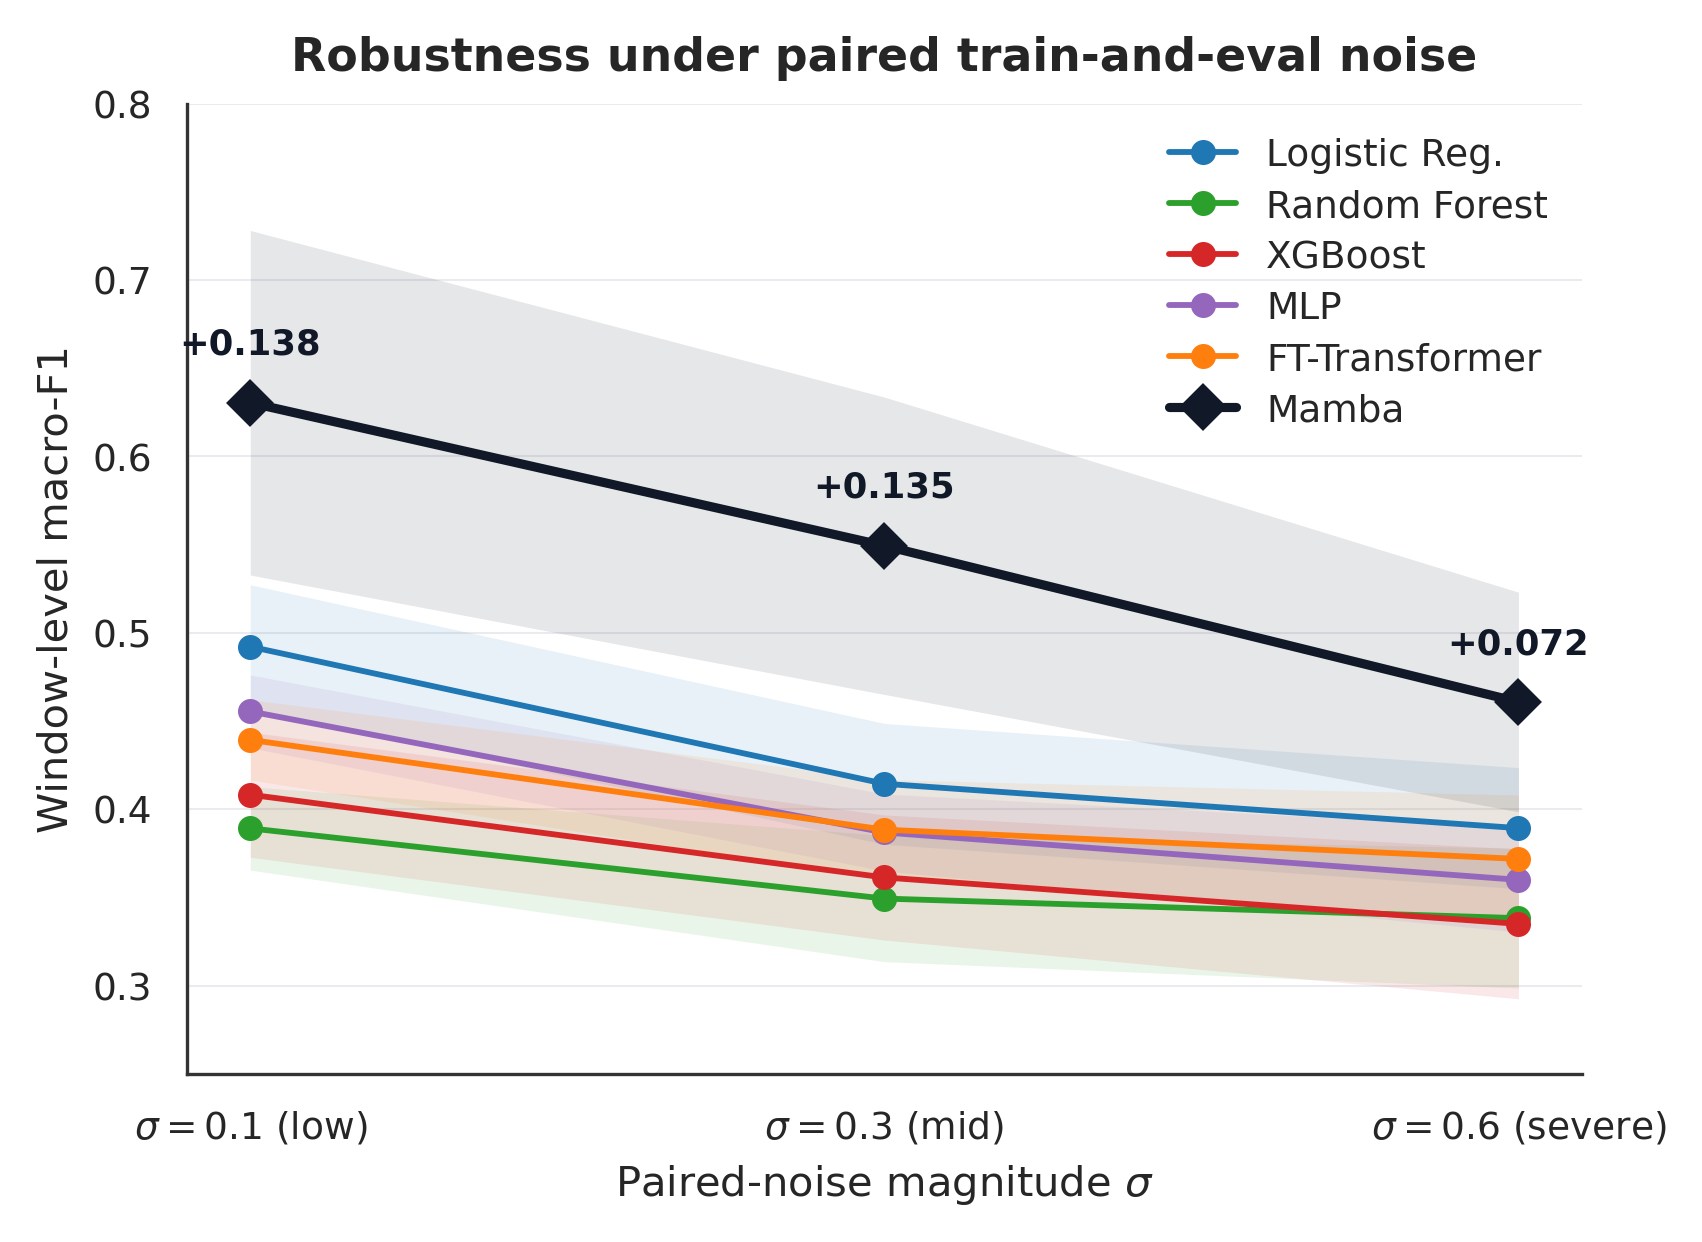
\includegraphics[width=0.9\linewidth]{../figures/fig3_robustness_curve.png}
\caption{Window-level macro-F1 versus paired-perturbation magnitude $\sigma \in \{0.1, 0.3, 0.6\}$ for all six models, under the paired-perturbation train-and-eval regime described in Section 3.4 (perturbation applied identically to training and validation features). Markers are fold means; the gap between Mamba and the strongest tabular baseline at each magnitude is annotated.}
\label{fig:robust}
\end{figure}

The Mamba sequence model retains its absolute lead across all three magnitudes: the window-F1 gap Mamba-vs-best-tabular is $0.138$ at $\sigma = 0.1$, $0.135$ at $\sigma = 0.3$, and $0.072$ at $\sigma = 0.6$. The gap narrows at severe perturbation, consistent with high-magnitude feature corruption progressively eroding the cross-window temporal signal that Mamba uniquely exploits --- as per-feature signal-to-corruption falls, per-window observations become less informative both for training and for inference, and the benefit of integrating them across time diminishes. The temporal-modeling advantage is bounded above by the signal present in the underlying features. All six models degrade monotonically from $\sigma = 0.1$ to $\sigma = 0.3$ to $\sigma = 0.6$, confirming the three magnitudes are genuine stress conditions. Because this protocol perturbs both training and evaluation features, the reported degradation reflects the combined cost of \emph{learning} from perturbed features and \emph{predicting} on perturbed features --- a learning-capacity test, not a post-hoc fragility test.

\begin{figure}[htbp]
\centering
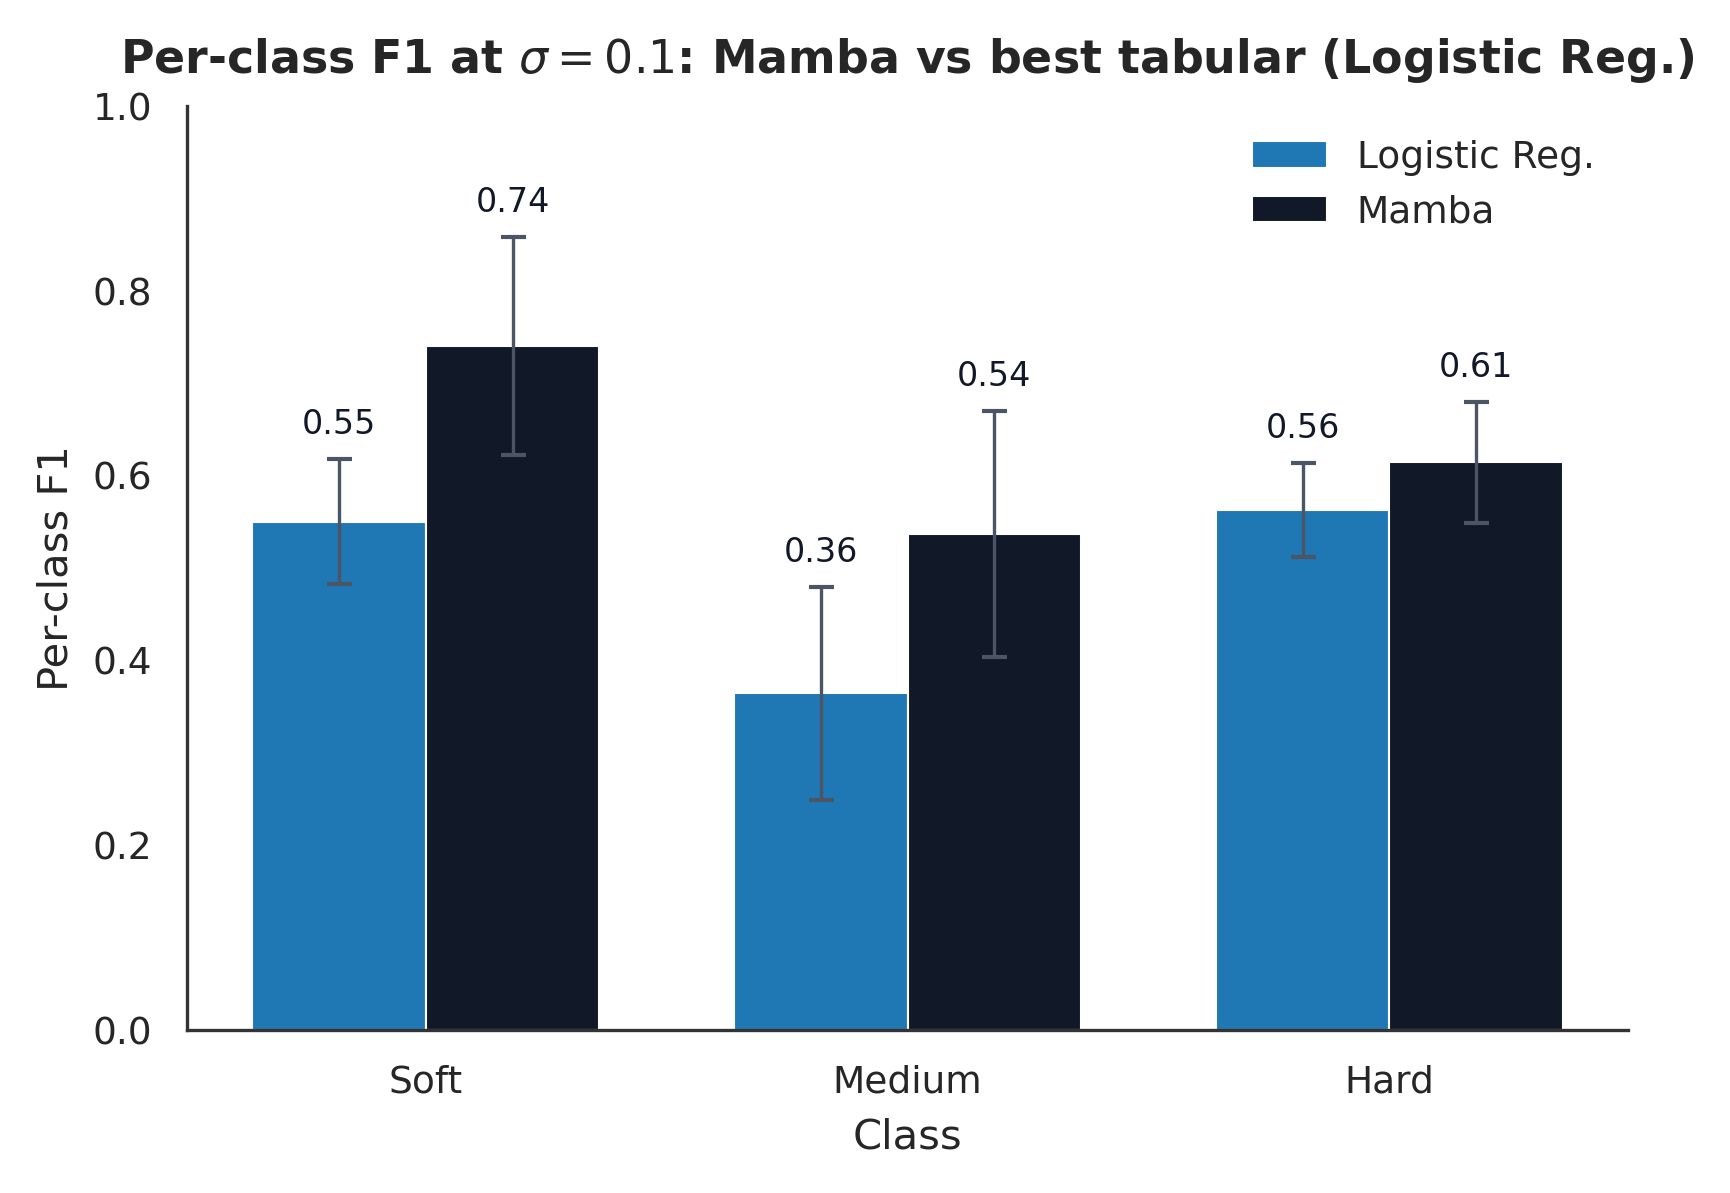
\includegraphics[width=0.9\linewidth]{../figures/fig5_per_class_f1_low.png}
\caption{Per-class F1 for each model at the $\sigma = 0.1$ regime, grouped by class (soft, medium, hard), with error bars equal to one standard deviation across folds.}
\label{fig:perclassf1}
\end{figure}

\begin{figure}[htbp]
\centering
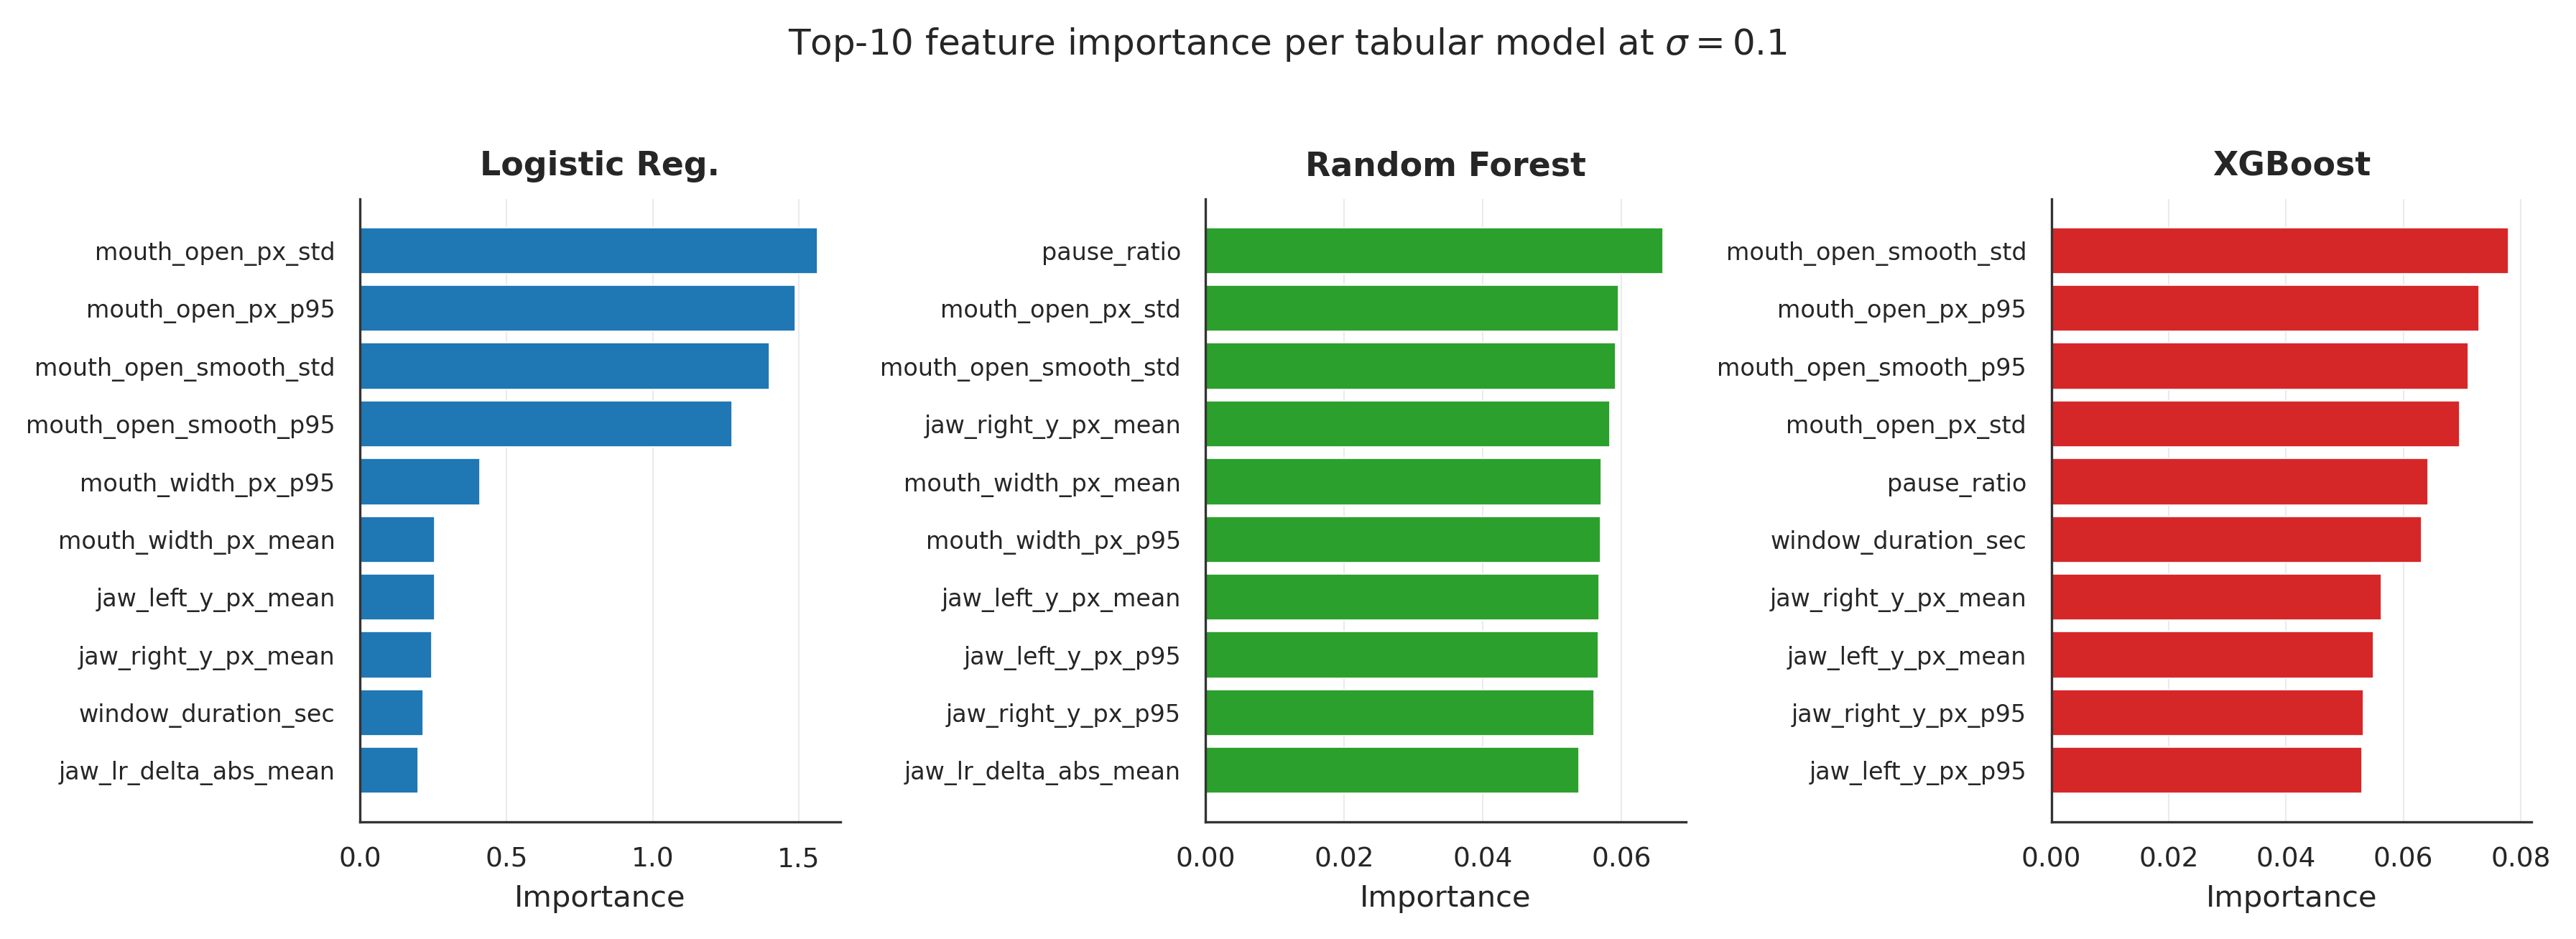
\includegraphics[width=0.9\linewidth]{../figures/fig4_feature_importance_top10.png}
\caption{Top-5 feature-importance bars for logreg, rf, and xgb, using the importances from Section 4.4.}
\label{fig:featimp}
\end{figure}

\subsection{Ablation: Mamba-3-style upgrades}

To quantify the contribution of the Mamba-3-style architectural refinements --- complex-valued $A$ and trapezoidal discretization --- we run a matched-size comparison between the hand-written hybrid and the vanilla Mamba-1 block from the \texttt{mamba-ssm} fused kernel, both at the reduced size of $d_\text{model} = 32$, $n_\text{blocks} = 1$, $d_\text{state} = 8$, with otherwise identical training hyperparameters and run for 30 epochs under the $\sigma = 0.1$ 5-fold CV.

\begin{table}[htbp]
\centering
\caption{Matched-size ablation: Mamba-3-style upgrades vs.\ vanilla Mamba-1 at $d_\text{model} = 32$, $n_\text{blocks} = 1$, $d_\text{state} = 8$, trained for 30 epochs at $\sigma = 0.1$. Window macro-F1 is fold mean $\pm$ std across 5 folds; chunk macro-F1 is fold mean.}
\label{tab:ablation}
\begin{tabular}{l r r}
\toprule
Variant & Window macro-F1 & Chunk macro-F1 \\
\midrule
Mamba-1 (real $A$, Euler, fused kernel) & $0.373 \pm 0.036$ & $0.446$ \\
Mamba-3-style (complex $A$, trapezoidal, hand-written) & $0.396 \pm 0.026$ & $0.492$ \\
$\Delta$ (upgraded $-$ Mamba-1) & $+0.023$ & $+0.046$ \\
\bottomrule
\end{tabular}
\end{table}

The complex-valued $A$ and trapezoidal-discretization upgrades yield a small but consistent improvement over the Mamba-1 baseline at matched size ($+0.023$ window-macro-F1, $+0.046$ chunk-macro-F1). At this smaller configuration, both variants converge in fewer epochs than the main model; we trained both for the same 30 epochs to isolate the architectural axis. A budget-matched comparison at 80 epochs and the full $d_\text{model} = 64$, $n_\text{blocks} = 2$, $d_\text{state} = 16$ configuration would further sharpen the comparison but lay outside the scope of this paper, primarily because of the wall-clock gap discussed next.

The hand-written implementation of the complex-$A$ selective scan is considerably more expensive than the fused Mamba-1 kernel: the same 5-fold $\times$ 30-epoch run takes approximately $613.4$ seconds for the hand-written hybrid versus $4.3$ seconds for the fused Mamba-1 baseline, a ratio of roughly $143\times$. This gap is implementation-driven, not algorithmic: the Mamba-1 baseline uses the official fused CUDA scan, whereas our hybrid with complex-valued $A$ and trapezoidal discretization falls back to a sequential Python scan because no fused CUDA kernel is publicly available for the complex-valued $A$ variant as of this writing. A bespoke CUDA implementation of the upgraded variant could close much of the cost gap. Given the current wall-clock cost, we use the standard Mamba-1 formulation in the main experiment and leave full-scale evaluation of the upgrades to future work.

The matched-size Mamba-1 vs. Mamba-3 ablation results are visualized in Figure \ref{fig:training}, plotting window- and chunk-level macro-F1 for both variants.

\begin{figure}[htbp]
\centering
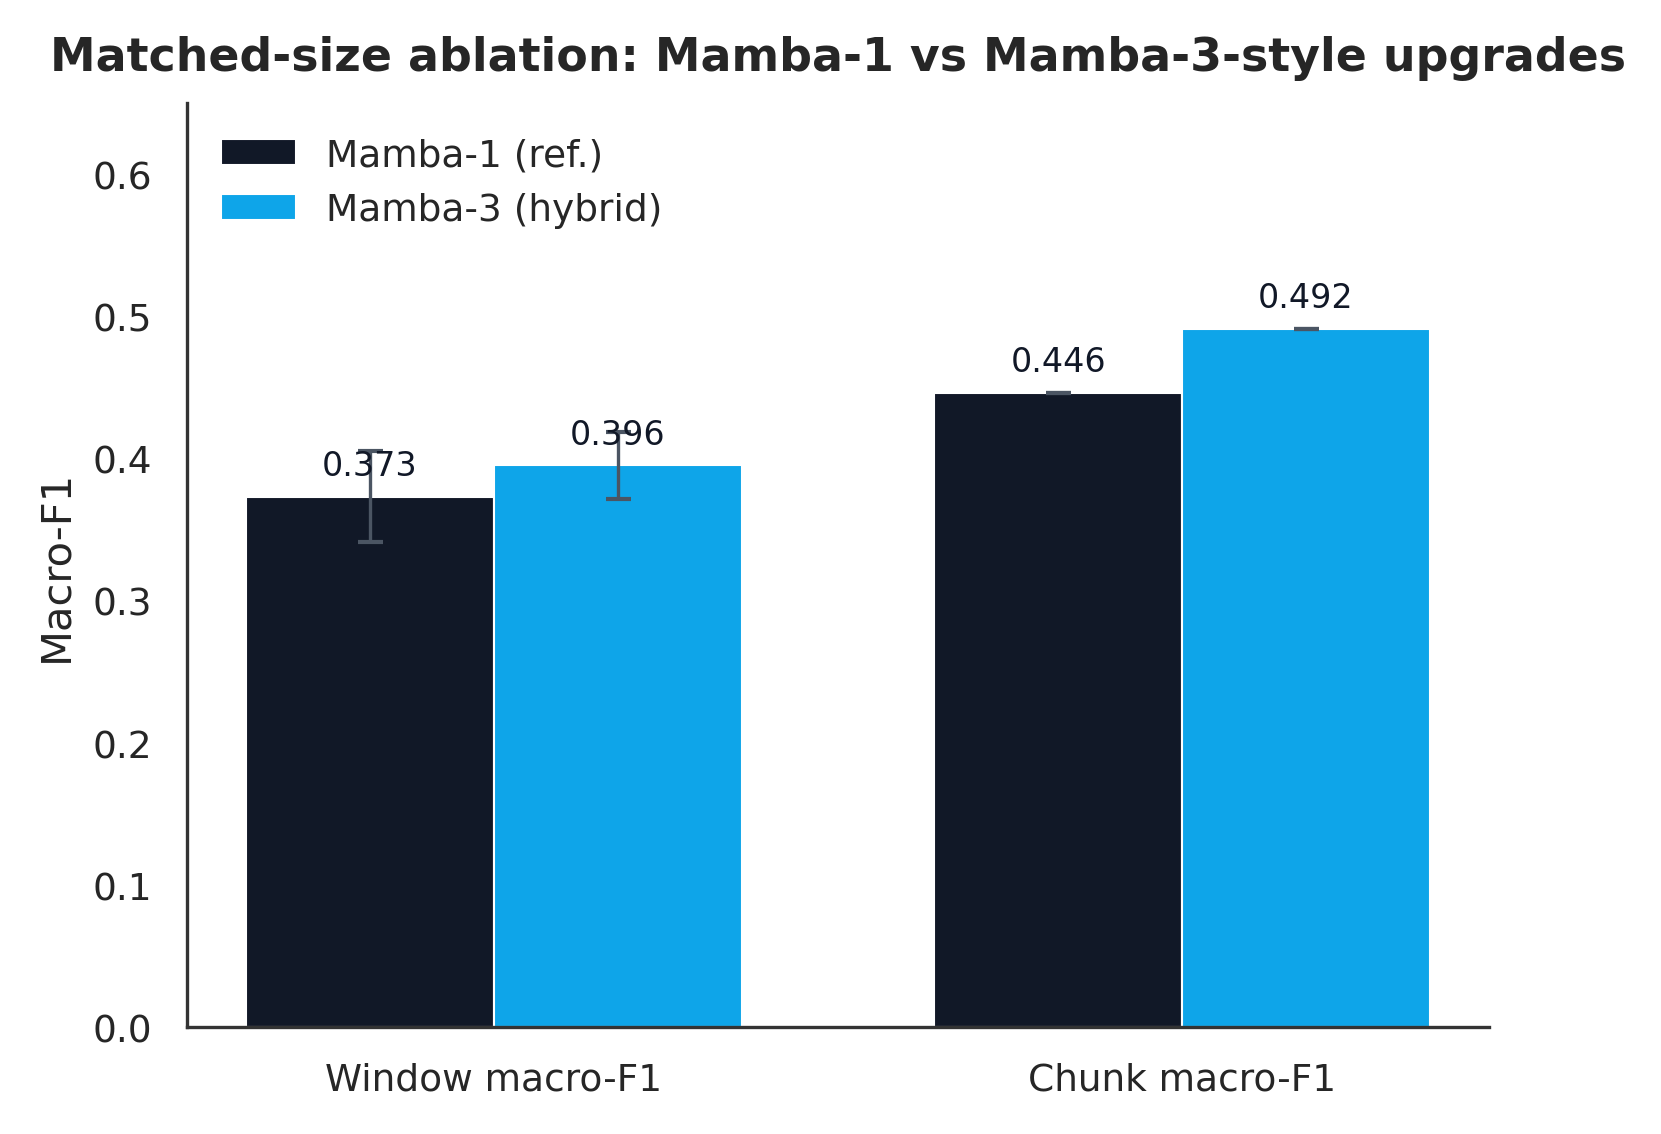
\includegraphics[width=0.9\linewidth]{../figures/fig6_ablation_mamba1_vs_mamba3.png}
\caption{Matched-size ablation comparison (Mamba-1 reference vs.\ Mamba-3 hybrid) at the tiny configuration ($d_{\text{model}}=32$, $n_{\text{blocks}}=1$, $d_{\text{state}}=8$, 30 epochs), window- and chunk-level macro-F1 on the $\sigma = 0.1$ regime.}
\label{fig:training}
\end{figure}

\section{Discussion and Limitations}

\textbf{What these results say about temporal modeling.} The headline result --- a $+0.138$ window-level macro-F1 gap between the sequence model and the strongest tabular baseline on the same per-window features --- supports the view that temporal dynamics are the dominant carrier of texture information in chewing-video feature sequences. A tabular classifier given only a per-window summary treats each window as independent evidence, ignoring exactly the structure (jaw-cycle periodicity, slow amplitude drift, pause sequencing) that most clearly discriminates texture. The paired-perturbation study in Section 4.5 strengthens this interpretation: the temporal-modeling advantage persists from $\sigma = 0.1$ (gap $0.138$) through $\sigma = 0.3$ (gap $0.135$) and remains positive at $\sigma = 0.6$ (gap $0.072$), the qualitative signature expected of a feature-exploiting inductive bias rather than a brittle optimization artifact. Whether a specifically \emph{selective} SSM is necessary --- as opposed to a bidirectional RNN, TCN, gated-recurrent baseline, or small Transformer --- is left to future work, flagged as a direct follow-up.

\textbf{On the chunk-level reversal.} Logistic regression narrowly beats Mamba on chunk-level macro-F1 ($0.685$ vs $0.652$) despite losing clearly on window-level. As discussed in Section 4.2, majority-vote aggregation grants a large boost to logreg ($+0.193$) relative to the modest boost it grants Mamba ($+0.022$), consistent with logreg's per-window errors being uncorrelated within a chunk while its per-window \emph{bias} points in the right direction on average. For pipelines whose decision rule is chunk-level majority vote, a well-regularized linear baseline remains competitive; deployment choices should weigh decision granularity against the learning-capacity advantages of the sequence model under perturbation.

\textbf{Limitations.} Several caveats apply.

\begin{enumerate}
    \item \textbf{Subject count.} The cohort contains 20 subjects, and the 5-fold protocol uses 4 subjects per validation fold --- a small experimental-unit count, leaving fold-to-fold variance wide. The Mamba window-F1 fold standard deviation of $0.098$, considerably larger than the tabular baselines' $0.02$--$0.035$, directly reflects this: some folds show dramatic improvement from the sequence model while others are much closer to tabular baseline performance, depending on which subjects are held out. Fold-mean numbers should be read as estimates, with the reported per-fold standard deviations as the relevant uncertainty; larger-cohort validation is a clear priority for any deployment claim.

    \item \textbf{Chunk boundaries.} Chunks are defined by the recording-session clip boundaries (Section 3.1); this means chunk-level majority-vote scoring is well-defined independently of the labels but it also inherits any artifacts present at the protocol joints, particularly when two adjacent chunks share a subject and camera setup. We did not explicitly penalize boundary-crossing confusions; a future study could quantify whether errors cluster at chunk edges and, if so, consider boundary-aware training.

    \item \textbf{Temporal resolution.} The current pipeline uses fixed-duration windows and treats the window-level feature sequence as the modeling granularity. Finer-grained frame-level modeling --- directly from the face-landmark time series, without the window-summary bottleneck --- is an obvious next step, and is a better match for the linear-time inference of selective SSMs.

    \item \textbf{Multi-modal fusion.} We did not explore audio, inertial, or explicit bite-instrumentation modalities, all of which carry complementary information about chewing and may be combinable with the visual pipeline at modest additional cost.

    \item \textbf{Cohort composition.} The cohort reflects the demographics and food items available in the study; generalization to other demographic groups, food types, and acquisition setups should be validated before any deployment claim is made.

    \item \textbf{Perturbation model.} The paired-perturbation study uses zero-mean Gaussian additive perturbation scaled per column and applied identically to training and evaluation features. This covers a natural class of sensor and landmark-detector measurement errors but does not model structured corruption such as missing frames, systematic bias, or adversarial manipulation; it also does not separate \emph{learning} fragility from \emph{test-time} fragility, which would require a crossed protocol (train clean / evaluate perturbed, and vice versa). These deserve separate study.

    \item \textbf{Ablation implementation.} The ${\sim}143\times$ wall-clock disadvantage of the hand-written complex-$A$ scan relative to the fused Mamba-1 kernel is an implementation artifact, not a fundamental property of the architecture; a fused kernel for complex-diagonal $A$ would make it feasible to test the Mamba-3-style upgrades at full scale rather than only at matched reduced size. Additionally, the matched-size ablation trains both variants for 30 epochs rather than the main model's 80; this keeps the architectural axis controlled but means the ablation numbers are not directly comparable to the main Mamba-1 row of Table \ref{tab:main}.

    \item \textbf{Sequence-baseline coverage.} We compare against tabular baselines only; we do not include alternative sequence families (e.g., GRU, TCN, small Transformer) because we did not run those experiments in this study. This leaves open whether the observed lead is specifically attributable to the selective-SSM inductive bias or would be matched by other sequence models. We flag this as a first-order follow-up item.

    \item \textbf{Single seed per fold.} Each fold is trained with a single seed (Section 3.3); multi-seed averaging would tighten the per-fold standard-deviation estimates and is a cheap and worthwhile extension.
\end{enumerate}

\section{Conclusion}

We studied whether a modern selective state-space model can improve food-texture classification from chewing-behavior video on the same per-window features as tabular baselines. Under a leave-subjects-out cross-validation protocol on a 20-subject cohort at the $\sigma = 0.1$ reference regime, a bidirectional Mamba-1 sequence model achieves a per-window macro-F1 of $0.630$, exceeding the strongest tabular baseline (logistic regression at $0.492$) by $+0.138$ points. On the chunk-level majority-vote metric the two are close, with logistic regression narrowly ahead ($0.685$ vs $0.652$); we report this as an honest caveat. Under a paired-perturbation train-and-eval regime with $\sigma \in \{0.1, 0.3, 0.6\}$ applied identically to training and validation features, the sequence model retains its absolute window-F1 lead over all tabular baselines at every magnitude, confirming that the advantage is a property of learning capacity rather than an artifact of a particular clean condition. A matched-size ablation of Mamba-3-style upgrades (complex-valued $A$, trapezoidal discretization) yields a small consistent gain ($+0.023$ window-F1) at roughly $143\times$ the wall-clock cost of the fused Mamba-1 kernel --- a gap driven by the absence of a fused CUDA implementation for complex-valued $A$ rather than by the architecture itself. Together, the results support temporal modeling as a cheap and effective addition to chewing-video feature pipelines, with further gains likely from finer temporal resolution, larger cohorts, alternative sequence-model families, fused kernels for newer SSM variants, and multi-modal fusion.

\begin{thebibliography}{99}

\bibitem{chen2016xgboost}
Chen, T.\ and Guestrin, C.
XGBoost: A Scalable Tree Boosting System.
In \emph{Proceedings of the 22nd ACM SIGKDD International Conference on Knowledge Discovery and Data Mining}, 2016.

\bibitem{dao2024mamba2}
Dao, T.\ and Gu, A.
Transformers are SSMs: Generalized Models and Efficient Algorithms through Structured State Space Duality (Mamba-2).
In \emph{Proceedings of the 41st International Conference on Machine Learning}, 2024.

\bibitem{mediapipe2022}
Google.
MediaPipe Face Landmarker.
Google Developers documentation, 2022.

\bibitem{gorishniy2021rtdl}
Gorishniy, Y., Rubachev, I., Khrulkov, V., and Babenko, A.
Revisiting Deep Learning Models for Tabular Data.
In \emph{Advances in Neural Information Processing Systems} 34, 2021.

\bibitem{gu2023mamba}
Gu, A.\ and Dao, T.
Mamba: Linear-Time Sequence Modeling with Selective State Spaces.
Preprint, 2023.

\bibitem{hairer1996}
Hairer, E.\ and Wanner, G.
\emph{Solving Ordinary Differential Equations II: Stiff and Differential-Algebraic Problems.}
Springer, 2nd edition, 1996.

\bibitem{hendrycks2019}
Hendrycks, D.\ and Dietterich, T.
Benchmarking Neural Network Robustness to Common Corruptions and Perturbations.
In \emph{International Conference on Learning Representations}, 2019.

\bibitem{loshchilov2019adamw}
Loshchilov, I.\ and Hutter, F.
Decoupled Weight Decay Regularization (AdamW).
In \emph{International Conference on Learning Representations}, 2019.

\bibitem{pedregosa2011sklearn}
Pedregosa, F.\ et al.
Scikit-learn: Machine Learning in Python.
\emph{Journal of Machine Learning Research}, 12, 2011.

\bibitem{szegedy2014}
Szegedy, C., Zaremba, W., Sutskever, I., Bruna, J., Erhan, D., Goodfellow, I., and Fergus, R.
Intriguing Properties of Neural Networks.
In \emph{International Conference on Learning Representations}, 2014.

\bibitem{vaswani2017attention}
Vaswani, A.\ et al.
Attention is All You Need.
In \emph{Advances in Neural Information Processing Systems} 30, 2017.

\end{thebibliography}

The complex-diagonal parameterization of $A$ and the trapezoidal discretization referenced in Section 3.2 are treated here as generic architectural refinements grounded in the classical diagonal-SSM and numerical-integration literatures; we attribute the individual building blocks to Gu and Dao (2023) \cite{gu2023mamba}, Dao and Gu (2024) \cite{dao2024mamba2}, and Hairer and Wanner (1996) \cite{hairer1996} rather than to any specific preprint whose authorship we cannot verify.

\appendix

\section{Hyperparameters and Per-Class Support}

\subsection{Hyperparameters and cross-validation}

\textbf{Optimizers.} All neural models use AdamW with cosine learning-rate annealing. Tabular NNs: learning rate $10^{-3}$, weight decay $10^{-4}$, batch size 256, 60 epochs for MLP and 30 for FT-Transformer. Mamba (main): learning rate $5 \times 10^{-4}$, weight decay $10^{-3}$, sequence batch size 4, 80 epochs, $d_\text{model} = 64$, $n_\text{blocks} = 2$, $d_\text{state} = 16$. Mamba (ablation, both variants): same optimizer settings but $d_\text{model} = 32$, $n_\text{blocks} = 1$, $d_\text{state} = 8$, trained for 30 epochs.

\textbf{Classical models.} Logistic regression: L2, \texttt{class\_weight="balanced"}, up to 3,000 iterations inside a \texttt{StandardScaler} pipeline. Random forest: 400 trees, no depth limit, balanced class weights, $n_\text{jobs}$ all cores. XGBoost: 400 trees, learning rate 0.05, max depth 6, row subsample 0.9, column subsample 0.9, multinomial soft-probability objective, histogram tree method.

\textbf{Cross-validation.} 5-fold StratifiedGroupKFold on \texttt{video\_id}, fallback to GroupKFold. Feature standardization (mean/std) fitted only on the training fold. Balanced class weights computed only on the training fold. Global random seed 42; per-fold seed is $42 + \text{fold\_index}$ for MLP, FT-Transformer, and Mamba; the classical models (logreg, rf, xgb) use seed 42 with no per-fold variation because their training is deterministic given the data order.

\subsection{Per-class support and per-class F1}

The dataset contains approximately 8,077 windows across 20 subjects, split into three classes. Per-class support is reported together with the per-class F1 of the main Mamba sequence model and of the strongest tabular baseline (logistic regression) at the $\sigma = 0.1$ (low-magnitude) regime in Table \ref{tab:perclass}. The logistic-regression per-class F1 values are read directly from the fold-mean row of the primary cross-validation output table at the low-magnitude regime; support counts are identical across models because they depend only on the OOF partition.

\begin{table}[htbp]
\centering
\caption{Per-class support and per-class F1 at the $\sigma = 0.1$ regime for the main Mamba sequence model and for the strongest tabular baseline (logistic regression), pooled over OOF predictions.}
\label{tab:perclass}
\begin{tabular}{l r r r}
\toprule
Class & Support & Per-class F1 (mamba) & Per-class F1 (logreg) \\
\midrule
soft & $503.8$ & $0.740$ & $0.550$ \\
medium & $584.6$ & $0.537$ & $0.364$ \\
hard & $527.0$ & $0.614$ & $0.563$ \\
\bottomrule
\end{tabular}
\end{table}

As noted in Section 4.3, medium is the hardest class for both models --- the expected behavior given that medium lies between its neighbors on the ordinal texture axis and inherits confusion mass from both sides. Soft and hard are recovered at comparable but distinctly higher rates by Mamba, with soft slightly higher. Logistic regression mirrors the same ordering --- soft and hard higher than medium --- but its per-class rates are uniformly lower, consistent with the $0.138$ gap in macro-F1. Figure \ref{fig:perclassf1} visualizes the same per-class pattern across all six models.

\subsection{Feature-importance top-5 (repeated for reference)}

For ease of reference, the top-5 feature importance rankings from Section 4.4 are repeated below. Figure \ref{fig:featimp} gives the same information as a bar chart.

\begin{itemize}
    \item \textbf{logreg} (absolute standardized coefficient magnitudes): \texttt{mouth\_open\_px\_std}, \texttt{mouth\_open\_px\_p95}, \texttt{mouth\_open\_smooth\_std}, \texttt{mouth\_open\_smooth\_p95}, \texttt{mouth\_width\_px\_p95}.
    \item \textbf{rf} (impurity-based importances): \texttt{pause\_ratio}, \texttt{mouth\_open\_px\_std}, \texttt{mouth\_open\_smooth\_std}, \texttt{jaw\_right\_y\_px\_mean}, \texttt{mouth\_width\_px\_mean}.
    \item \textbf{xgb} (impurity-based importances): \texttt{mouth\_open\_smooth\_std}, \texttt{mouth\_open\_px\_p95}, \texttt{mouth\_open\_smooth\_p95}, \texttt{mouth\_open\_px\_std}, \texttt{pause\_ratio}.
\end{itemize}

\subsection{Figure captions}

Each figure is referenced explicitly in the body of the paper. Figure \ref{fig:pipeline} is referenced in Section 4.1 (Table \ref{tab:main} caption); Figure \ref{fig:confusion} in Section 4.3; Figure \ref{fig:robust} in Section 4.5; Figure \ref{fig:perclassf1} in Section 4.3 and Appendix A.2; Figure \ref{fig:featimp} in Section 4.4 and Appendix A.3; Figure \ref{fig:training} in Section 4.6.

\end{document}
